% Chapter Template

\chapter{Optimization on Structures} % Main chapter title
\label{Chapter5} % Change X to a consecutive number; for referencing this chapter elsewhere, use \ref{ChapterX}
\lhead{Chapter 5. \emph{Optimization on Structures}} % Change X to a consecutive number; this is for the header on each page - perhaps a shortened title



\rule{\textwidth}{0.4pt} \\[0.5cm]
\textit{``For the things we have to learn before we can do them, we learn by doing them"}

\begin{flushright}
Aristotle
\end{flushright}
\rule{\textwidth}{0.4pt} 

%----------------------------------------------------------------------------------------
%	SECTION 1
%----------------------------------------------------------------------------------------
\section{Optimzation on Graphs}

\subsection{Max-product (Loopy) Belief Propagation}
\begin{algorithm}
	\caption{Belief Propagation for tree-structured Markov networks}
	\label{alg:BP_tree}
\begin{algorithmic}[1]
\STATE  select one variable as the root; 
\STATE  starting from all leaves, propagate \emph{beliefs} toward the root as:
\begin{equation*}
m_{i \rightarrow j}(x_j)= \sum_{x_i}\left\{\phi(x_i,x_j) \prod_{k\in \text{Ne}(i)\backslash j} m_{k \rightarrow i}(x_i)\right\}
\end{equation*}
\STATE  when the root receives all messages from its neighbors, then propagate backwards the \emph{``inverse beliefs"} as the step 2;
\STATE  the marginal probability of each variable is computed as: 
\begin{equation*}
P(x_i)\propto \prod_{k\in \text{Ne}(i)} m_{k \rightarrow i}(x_i)
\end{equation*}
where Ne$(i)$ denotes the neighboring variables of $x_i$ in the graph. 
\end{algorithmic}
\end{algorithm}

\begin{algorithm}
	\caption{Generalized Belief Propagation for Loopy Markov networks}
	\label{alg:LBP}
\begin{algorithmic}[1]
%\STATE  In a loopy graph, there is no root and leaves because of loop.
\STATE  initialize all messages $m_{i\rightarrow j}$ in both directions of all connected variables randomly or with a constant value (\emph{e.g.} 1);
\WHILE {all messages converge}
\STATE  update messages as:
\begin{equation*}
  m^{(t+1)}_{i \rightarrow j}(x_j)= \sum_{x_i}\left\{\phi(x_i,x_j) \prod_{k\in \text{Ne}(i)\backslash j} m^{(t)}_{k \rightarrow i}(x_i)\right\}
\end{equation*}
\ENDWHILE
\end{algorithmic}
\end{algorithm}


\subsection{Iterated Conditional Mode}
\subsection{Graph Cut}

\section{Optimization on Matrix Manifolds}

\subsection{3D Point Cloud Registration with Convex Optimization on SO(3) Manifold}
3D shape pose estimation is an essential in computer vision and robot
perception.
Unitl now, the poses of 3D shapes are usually estimated by using registration algorithms. 
Despite intensive study, 3D shape
registration remains an open question. 
For most existing registration algorithms, there are many obstacles to
practical use them in fully autonomous systems. For instance, ICP usually
requires manual assistance to provide a good initialization, and
Gaussian Mixtures and SoftAssign are too expensive for real-time
tasks. Therefore, a novel algorithm was developed by the author and co-workers to satisfy the
practical need for better robustness and higher efficiency. Quite
different from previous registration methods, instead of computing
correspondence and alignment in 3D space, the propsed algorithm first map
points to a higher, possibly infinite-dimensional space by applying
Kernel methods. Registration is subsequently performed within feature
space by aligning corresponding principal components. The result is
projected back into 3D pose space. The whole procedure is
theoretically elegant and efficient. Kernel PCA is used to avoid
explicit computation in feature space, and SE(3) on-manifold
optimization is employed to enhance the generality of our registration algorithm. 
Empirical results demonstrate that the proposed method is quite accurate
and robust to various challenging circumstances (\emph{e.g.} large motion,
presence of outliers), and remarkably, it is much faster than other
state-of-the-art methods with comparable performance. 

\begin{shaded}
 {\Huge IX.} \textbf{Hanchen Xiong}, Sandor Szedmak, Justus Piater {\it Efficient, General Point Cloud Registration With Kernel Feature Maps}, 
In Proceedings of 10th International Conference on Computer and Robot Vision (CRV13), pp 83-90, 2013, IEEE.
\end{shaded}
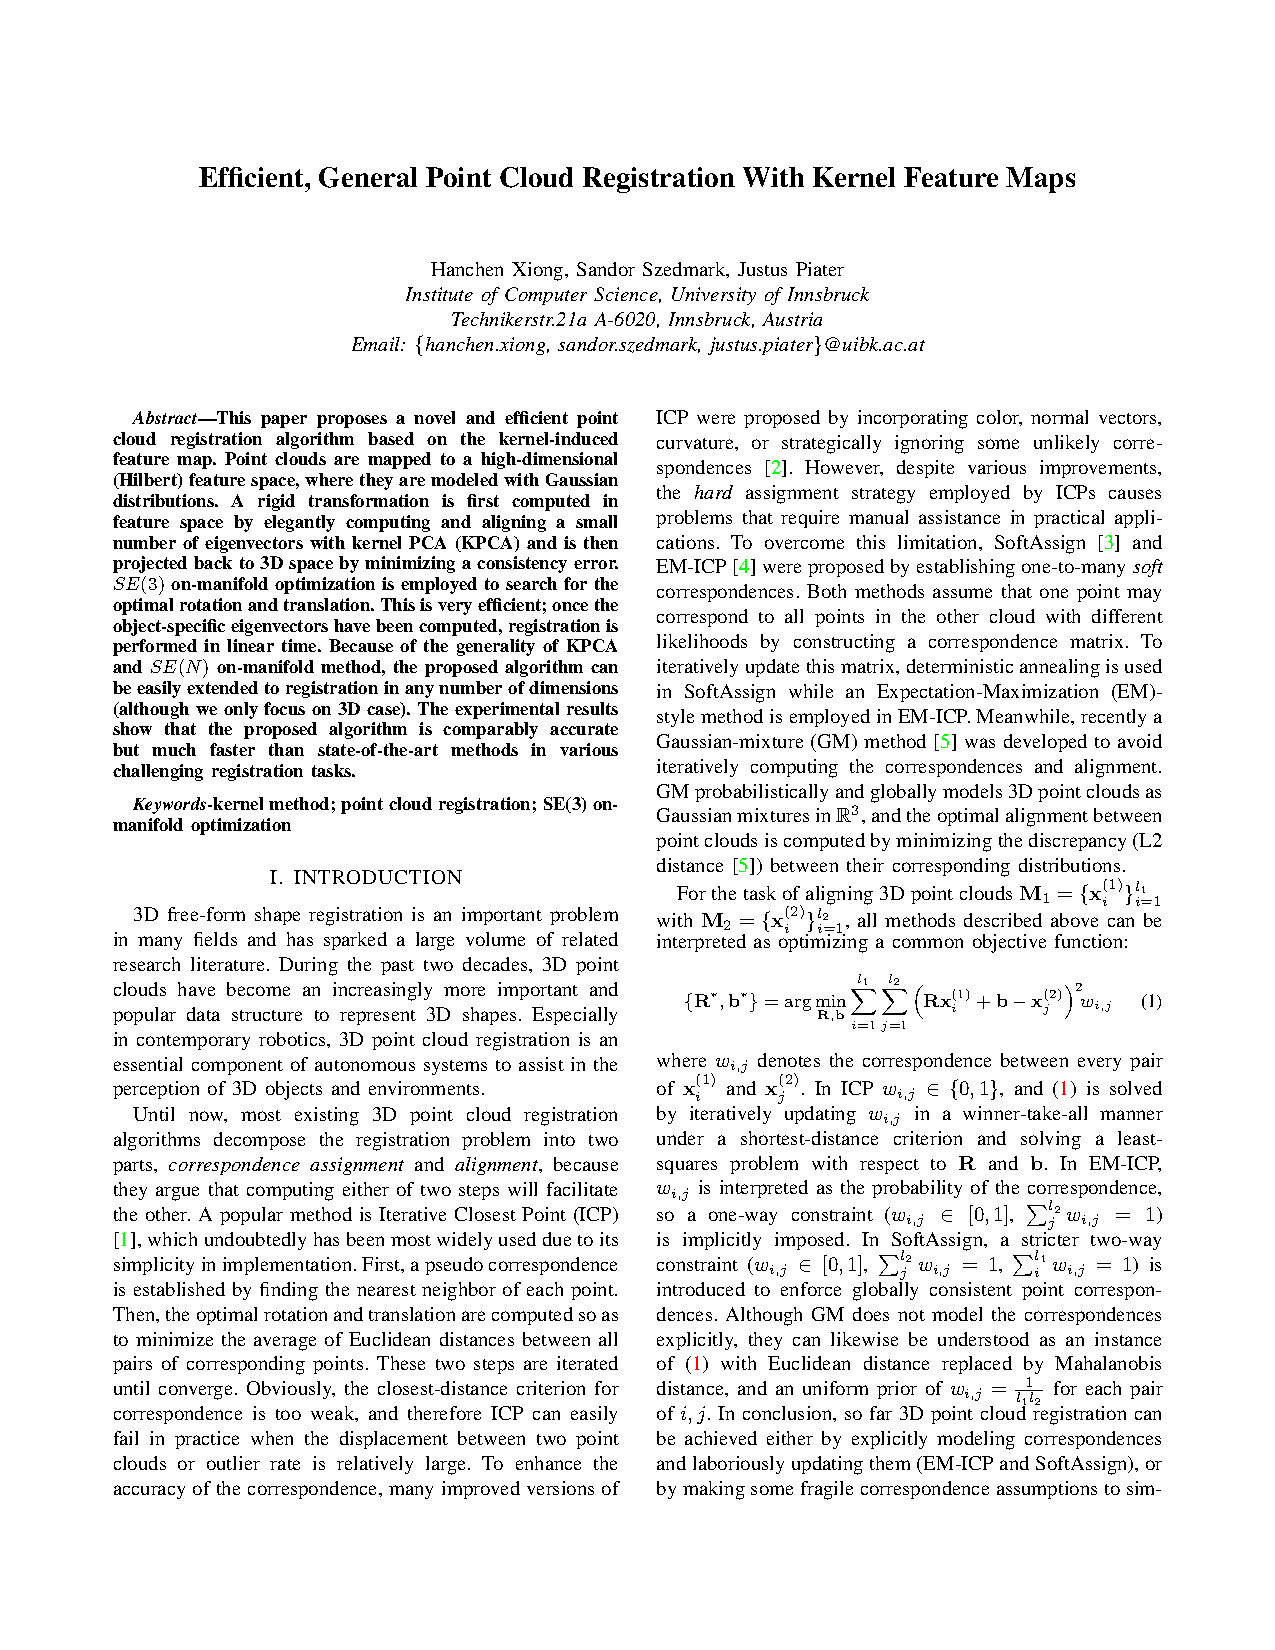
\includepdf[offset=3cm -3cm, scale=1, pages=-,pagecommand={\pagestyle{fancy}}]{./Papers/Xiong-2013-CRV.pdf}


%----------------------------------------------------------------------------------------
%	SECTION 2
%----------------------------------------------------------------------------------------



%\section{Stochastic Optmization of Black-box Functions on Riemannian Manifolds using Kernel Adaptive Sequential Monte Carlo}
%
%Sed ullamcorper quam eu nisl interdum at interdum enim egestas. Aliquam placerat justo sed lectus lobortis ut porta nisl porttitor. Vestibulum mi dolor, lacinia molestie gravida at, tempus vitae ligula. Donec eget quam sapien, in viverra eros. Donec pellentesque justo a massa fringilla non vestibulum metus vestibulum. Vestibulum in orci quis felis tempor lacinia. Vivamus ornare ultrices facilisis. Ut hendrerit volutpat vulputate. Morbi condimentum venenatis augue, id porta ipsum vulputate in. Curabitur luctus tempus justo. Vestibulum risus lectus, adipiscing nec condimentum quis, condimentum nec nisl. Aliquam dictum sagittis velit sed iaculis. Morbi tristique augue sit amet nulla pulvinar id facilisis ligula mollis. Nam elit libero, tincidunt ut aliquam at, molestie in quam. Aenean rhoncus vehicula hendrerit.
%
%
%
